%@TheDoctorRAB
%standard white paper/preproposal format
%
%%%%%
%
%REFERENCES
%
%neup.bst - numbered citations in order of appearance, short author list with et al in reference section
%nsf.bst - numbered citations in order of appearance, full author list in references section
%standard.bst - citations with author last name with et al for more than 2 authors; full author list in references section
%ans.bst is for ANS only. 
%
%author = {Lastname, Firstname and Lastname, Firstname and Lastname, Firstname} for all bst formats
%bst renders the author list itself
%
%author = {{Nuclear Regulatory Commission}} if the author is an organization, institution, etc., and not people
%
%title = {{}} for all
%
%for all - use \citep{-} - [1] or (Borrelli, 2021) in the text
%standard.bst \cite{-} - Borrelli (2021) in the text
%standard.bst lists references alphabetically
%the rest list numerically
%
%
%%% slides 
%
%\citep{xxxnna} where the citation should go
%\blfootnote{\fontsize\cite{xxxnna}\fontsize\bibentry{xxxnna}} before \end{frame}
%
%
%%%%%

%%%%% presentation settings
\documentclass[aspectratio=1610,pdftex,dvipsnames,compress,xcolor={dvipsnames}]{beamer}
\usetheme{Boadilla}
\usecolortheme{seahorse}
\beamertemplatenavigationsymbolsempty
\addtobeamertemplate{footnote}{\hskip -2em}{} %pushes footnote to margin
\setbeamerfont{title}{series=\bfseries}
\setbeamertemplate{page number in head/foot}[framenumber] %just gives slide number; comment out for 1/7, 2/7...
\definecolor{BackGround}{RGB}{255,250,240}
\setbeamercolor{background canvas}{bg=BackGround}
%%%%%


%%%%% general 
%\documentclass[11pt,a4paper]{article}
%\usepackage[lmargin=1in,rmargin=1in,tmargin=1in,bmargin=1in]{geometry}
\usepackage[pagewise]{lineno} %line numbering
\usepackage{setspace}
\usepackage{ulem} %strikethrough - do not \sout{\cite{}}
\usepackage{graphicx}
\usepackage{mypythonhighlight,verbatim}
\usepackage{filecontents}
\usepackage{tablefootnote}
\usepackage{footnotehyper}
\usepackage{float}
%\usepackage{subfig}
\usepackage[yyyymmdd]{datetime} %date format
\renewcommand{\dateseparator}{.}
\graphicspath{{img/}} %path to graphics
\setcounter{secnumdepth}{5} %set subsection to nth level
\usepackage{needspace}
\usepackage[stable,hang,flushmargin]{footmisc} %footnotes in section titles and no indent; standard.bst
\usepackage[inline]{enumitem}
\setlist[itemize]{label=\textbullet}
\usepackage{boldline}
\usepackage{makecell}
\usepackage{booktabs}
\usepackage{amssymb}
\usepackage{gensymb}
\usepackage{amsmath,nicefrac}
\usepackage{physics}
\usepackage{lscape}
\usepackage{array}
\usepackage{chngcntr}
\usepackage{hyperref}
\hypersetup{colorlinks,linkcolor=black,citecolor=black,urlcolor=blue} 
%\usepackage{sectsty}
\usepackage{textcomp}
\usepackage{lastpage}
\usepackage{xargs} %for \newcommandx
\usepackage[colorinlistoftodos,prependcaption,textsize=tiny]{todonotes} %makes colored boxes for commenting
\usepackage{soul}
\usepackage{color}
\usepackage{marginnote}
\usepackage[figure,table]{totalcount}
\usepackage[capitalise]{cleveref}
\usepackage{microtype} %improves typography for pdf
\usepackage[pdftex,dvipsnames]{colortbl} %change font color
%%%%%


%%%%% tikz
\usepackage{pgf}
\usepackage{tikz} % required for drawing custom shapes
\usetikzlibrary{shapes,arrows,automata,trees}
%%%%%


%%%%% fonts
\usepackage{times}
%\renewcommand{\sfdefault}{ubuntu}
%arial - uncomment next two lines
%\usepackage{helvet}
%\renewcommand{\familydefault}{\sfdefault}
%%%%%


%%%%% references
%\usepackage[round,semicolon]{natbib} %for (Borrelli 2021; Clooney 2019) - standard.bst 
\usepackage[numbers,sort&compress]{natbib} %for [1-3] - nsf.bst, neup.bst
\setlength{\bibsep}{7pt} %sets space between references
%\renewcommand{\bibsection}{} %suppresses large 'references' heading
%\renewcommand\bibpreamble{\vspace{\baselineskip}} %sets spacing after heading if not using default references heading
%%%%%


%%%%% tables and figures
\usepackage{longtable} %need to put label at top under caption then \\ - use spacing
\usepackage{tablefootnote}
\usepackage{tabularx}
\usepackage{multirow}
\usepackage{tabto} %general tabbed spacing
\usepackage{pdfpages}
\usepackage{wrapfig} %wraps figures around text
\setlength{\intextsep}{0.00mm}
\setlength{\columnsep}{1.00mm}
\usepackage[singlelinecheck=false,labelfont=bf]{caption}
\usepackage{subcaption}
\captionsetup[table]{justification=justified,skip=5pt,labelformat={default},labelsep=period,name={Table}} %sets a space after table caption
\captionsetup[figure]{justification=justified,skip=5pt,labelformat={default},labelsep=period,name={Figure}} %sets space above caption, 'figure' format
\captionsetup[wrapfigure]{justification=centering,aboveskip=0pt,belowskip=0pt,labelformat={default},labelsep=period,name={Fig.}} %sets space above caption, 'figure' format
\captionsetup[wraptable]{justification=centering,aboveskip=0pt,belowskip=0pt,labelformat={default},labelsep=period,name={Table}} %sets space above caption, 'figure' format
%%%%%


%%%%% watermark
%\usepackage[firstpage,vpos=0.63\paperheight]{draftwatermark}
%\SetWatermarkText{\shortstack{DRAFT\\do not distribute}}
%\SetWatermarkScale{0.20}
%%%%%


%%%%% cross referencing files
%\usepackage{xr} %for revisions - will cross reference from one file to here
%\externaldocument{/path/to/auxfilename} %aux file needed
%%%%%


%%%%% toc and glossaries
\usepackage[toc,title]{appendix}
\usepackage[acronym,nomain,nonumberlist]{glossaries}
\makenoidxglossaries
%\usepackage{titlesec,titletoc}
%\renewcommand{\thepart}{ARTICLE \Roman{part}} %puts the label into the command so \thelabel will carry through
%\renewcommand{\thesection}{\arabic{section}} %puts the label into the command so \thelabel will carry through
%\titleformat{\part}{\normalfont\large\bfseries}{\thepart}{}{}[]
%\titlespacing*\part{0pt}{0.95\baselineskip}{0.75\baselineskip}
%\titleformat{\section}[runin]{\normalfont\large\bfseries}{\thesection}{-1em}{}[.]
%\titlespacing*\section{0pt}{0.65\baselineskip}{0.55\baselineskip}
%\titleformat{\subsection}[runin]{\normalfont\normalsize\bfseries}{\thesubsection}{-1em}{}[.]
%\titlespacing*\subsection{0pt}{0.50\baselineskip}{0.35\baselineskip}
%\titleformat{\paragraph}[runin]{\normalfont\normalsize\bfseries\itshape}{\theparagraph}{-1em}{}[.]
%\titlespacing*\paragraph{0pt}{0.45\baselineskip}{0.25\baselineskip}
%\titleformat{\subparagraph}[runin]{\normalfont\normalsize\itshape}{\thesubparagraph}{-1em}{}[.]
%\titlespacing*\subparagraph{0pt}{0.40\baselineskip}{0.25\baselineskip}
%\titleformat{\paragraph}[hang]{\normalfont\normalsize\bfseries}{\theparagraph}{5pt}{}[]
%\titlespacing*\paragraph{0pt}{0.50\baselineskip}{0.25\baselineskip}
%\titleformat{\subparagraph}[runin]{\normalfont\normalsize\itshape}{\thesubparagraph}{-1em}{}[.]
%\titlespacing*\subparagraph{0pt}{0.40\baselineskip}{0.20\baselineskip}
%%%%%


%%%%% editing
\newcommand{\edit}[1]{\textcolor{blue}{#1}} %shortcut for changing font color on revised text
\newcommand{\fn}[1]{\footnote{#1}} %shortcut for footnote tag
\newcommand*\sq{\mathbin{\vcenter{\hbox{\rule{.3ex}{.3ex}}}}} %makes a small square as a separator $\sq$
%\newcommand{\sk}[1]{\sout{#1}} %shortcut for default strikethrough - do not sk through citep
\newcommand\sk{\bgroup\markoverwith{\textcolor{red}{\rule[0.5ex]{1pt}{1pt}}}\ULon} %strikethrough with red line; not in \section{}
%\st{} does strikethrough using soul package but does not like acronyms
\newcommand{\blucell}{\cellcolor{aliceblue}} %use to shade in table cell
\newcommand{\grycekk}{\cellcolor{lightgray}} %use to shade in table cell
\newcommand{\whicell}{\cellcolor{antiquewhite}} %use to shade in table cell
%%%%%


%%%%% colors
%http://latexcolor.com/
%https://en.wikibooks.org/wiki/LaTeX/Colors#:~:text=black%2C%20blue%2C%20brown%2C%20cyan,be%20available%20on%20all%20systems.
\definecolor{aliceblue}{rgb}{0.94, 0.97, 1.0}
\definecolor{antiquewhite}{rgb}{0.98, 0.92, 0.84}
\definecolor{lightmauve}{rgb}{0.86, 0.82, 1.0}
\definecolor{brilliantlavender}{rgb}{0.96, 0.73, 1.0}
\definecolor{brandeisblue}{rgb}{0.0, 0.44, 1.0}
\definecolor{darkmidnightblue}{rgb}{0.0, 0.2, 0.4}

\newcommand{\x}{\cellcolor{aliceblue}} %use to shade in table cell
\newcommand{\y}{\cellcolor{lightgray}} %use to shade in table cell
\newcommand{\z}{\cellcolor{antiquewhite}} %use to shade in table cell
%%%%%


%%%%% acronyms
\newcommand{\acf}{\acrfull} %full acronym
\newcommand{\acl}{\acrlong} %long acronym
\newcommand{\acs}{\acrshort} %short acronym

\newcommand{\acfp}{\acrfullpl} %full acronym plural
\newcommand{\aclp}{\acrlongpl} %long acronym plural
\newcommand{\acsp}{\acrshortpl} %short acronym plural
%%%%%


%%%%% todonotes
\newcommandx{\cmt}[2][1=]{\todo[author=\textbf{STRUCTURE},tickmarkheight=0.15cm,linecolor=red,backgroundcolor=red!25,bordercolor=black,#1]{#2}}
\newcommandx{\con}[2][1=]{\todo[author=\textbf{CONTENT},tickmarkheight=0.15cm,linecolor=brilliantlavender,backgroundcolor=brilliantlavender,bordercolor=black,#1]{#2}}
\newcommandx{\rab}[2][1=]{\todo[noline,author=\textbf{RAB},backgroundcolor=Plum!25,bordercolor=black,#1]{#2}}


%\newcommandx{\jon}[2][1=]{\todo[noline,author=\textbf{ATTN: Johnson},backgroundcolor=blue!25,bordercolor=black,#1]{#2}}
%\newcommandx{\han}[2][1=]{\todo[noline,author=\textbf{ATTN: Haney},backgroundcolor=OliveGreen!25,bordercolor=black,#1]{#2}}
%\newcommandx{\rab}[2][1=]{\todo[author=\textbf{RAB},tickmarkheight=0.15cm,linecolor=Plum,backgroundcolor=Plum!25,bordercolor=black,#1]{#2}}
%\newcommandx{\han}[2][1=]{\todo[author=\textbf{ATTN: Haney},tickmarkheight=0.15cm,linecolor=OliveGreen,backgroundcolor=OliveGreen!25,bordercolor=OliveGreen,#1]{#2}}
%\newcommandx{\jon}[2][1=]{\todo[author=\textbf{ATTN: Johnson},tickmarkheight=0.15cm,linecolor=blue,backgroundcolor=blue!25,bordercolor=blue,#1]{#2}}


% highlighting 
\DeclareRobustCommand{\hlc}[1]{{\sethlcolor{LimeGreen}\hl{#1}}}
\makeatletter
    \if@todonotes@disabled
    \newcommand{\hlh}[2]{#1}
    \else
    \newcommand{\hlh}[2]{\han{#2}\hlc{#1}}
    \fi
    \makeatother

\DeclareRobustCommand{\hld}[1]{{\sethlcolor{CornflowerBlue}\hl{#1}}}
\makeatletter
    \if@todonotes@disabled
    \newcommand{\hlj}[2]{#1}
    \else
    \newcommand{\hlj}[2]{\jon{#2}\hld{#1}}
    \fi
    \makeatother

\DeclareRobustCommand{\hlf}[1]{{\sethlcolor{lightmauve}\hl{#1}}}
\makeatletter
    \if@todonotes@disabled
    \newcommand{\hlb}[2]{#1}
    \else
    \newcommand{\hlb}[2]{\rab{#2}\hlf{#1}}
    \fi
    \makeatother
%%%%%


%%%%% table alignments
\newcolumntype{L}[1]{>{\raggedright\let\newline\\\arraybackslash\hspace{0pt}}m{#1}} %uses \raggedright with m,p{} in table column
\newcolumntype{C}[1]{>{\centering\let\newline\\\arraybackslash\hspace{0pt}}m{#1}} %uses \raggedright with m,p{} in table column
\newcolumntype{R}[1]{>{\raggedleft\let\newline\\\arraybackslash\hspace{0pt}}m{#1}} %uses \raggedright with m,p{} in table column
%%%%%


%%%%% table contents
\makeatletter
\renewcommand\tableofcontents{%
    \@starttoc{toc}%
}
\makeatother

\makeatletter
\renewcommand\listoffigures{%
    \@starttoc{lof}%
}
\makeatother

\makeatletter
\renewcommand\listoftables{%
    \@starttoc{lot}%
}
\makeatother

\makeatletter
\newcommand*\ftp{\fontsize{16.5}{17.5}\selectfont}
\makeatother
%%%%%


%%%%% user commands
\newcommand\blfootnote[1]{%
  \begingroup
  \renewcommand\thefootnote{}\footnote{#1}%
  \addtocounter{footnote}{-1}%
  \endgroup
}

\makeatletter
\renewcommand{\@biblabel}[1]{#1.\hfill} %bibliography ordered list has numbers left flush
\makeatother
%%%%%

%%%%% archived section commands - use titlesec
%\makeatletter
%\renewcommand\section{%
%    \@startsection{section}{1}{\z@ }{0.50\baselineskip}{0.25\baselineskip}
%    {\large \normalfont \bfseries}}%

%\makeatletter
%\renewcommand\paragraph{%
%    \@startsection{paragraph}{4}{\z@ }{0.55\baselineskip}{-1em}
%    {\normalfont \normalsize \bfseries}}%

%\makeatletter
%\renewcommand\subparagraph{%
%    \@startsection{subparagraph}{5}{\z@ }{0.40\baselineskip}{-1em}
%    {\normalfont \normalsize \itshape }}%

%\makeatletter
%\renewcommand\subsection{%
%    \@startsection{subsection}{2}{\z@ }{0.45\baselineskip}{0.25\baselineskip}
%    {\large \normalfont \bfseries}}%
%%%%%


%%%%% header and footer
%\usepackage{fancyhdr}
%\pagestyle{fancy}
%\fancyhf{} %move page number to bottom right
%\renewcommand{\headrulewidth}{0pt} %set line thickness in header; uncomment as is to remove line
%\lhead{\scriptsize Name}
%\lhead{\scriptsize PNUCENE-D-22-xxxxx}
%\chead{\scriptsize \textit{PhD White Paper Project Proposal}}
%\rhead{\scriptsize \today}
%\rfoot{\thepage}
%%%%%


%%%%%%% citations
%\begin{filecontents}{references.bib}
%\end{filecontents}
%%%%%%%


%%%%% acronyms
% alphabetical ordering is automated
\newacronym{nrs}{NRHES}{Nuclear Renewable Hybrid Energy System}
\newacronym{ahp}{AHP}{Analytical Hierarchy Process}
\newacronym{inl}{INL}{Idaho National Laboratory}
\newacronym{orl}{ORNL}{Oak Ridge National Laboratory}
\newacronym{anl}{ANL}{Argonne National Laboratory}
\newacronym{npp}{NPP}{Nuclear Power Plant}
\newacronym{smr}{SMR}{Small Modular Reactor}
\newacronym{ump}{UAMPS}{Utah Associated Municipal Power Systems}
\newacronym{nus}{NuScale}{NuScale Power, LLC}
\newacronym{nrc}{NRC}{United States Nuclear Regulatory Commission}
\newacronym{epri}{EPRI}{Electric Power Research Institute}
\newacronym{nerc}{NERC}{North American Electric Reliability Corporation}
\newacronym{ci}{CI}{Consistency Index}
\newacronym{cr}{CR}{Consistency Ratio}
\newacronym{htse}{HTSE}{High Temperature Steam Electrolysis}
\newacronym{lwr}{LWR}{Light Water Reactor}
\newacronym{eia}{EIA}{U.S. Energy Information Administration}
\newacronym{oer}{OER}{Online Educational Resource}
\newacronym{lms}{LMS}{Learning Management System}
\newacronym{cps}{CPS}{Cyber-Physical Systems}
\newacronym{nsf}{NSF}{National Science Foundation}
\newacronym{wsc}{WSC}{Western Services Corporation}
\newacronym{cae}{CAES}{Center for Advanced Energy Studies}
\newacronym{hsl}{HSSL}{Human System Simulation Laboratory}
\newacronym{pwr}{PWR}{Pressurized Water Reactor}
\newacronym{bwr}{BWR}{Boiling Water Reactor}
\newacronym{roi}{ROI}{Return on Investment}
\newacronym{ic}{I\&C}{Instrumentation \& Controls}
\newacronym{mwe}{MWe}{Megawatts-electric}
\newacronym{ics}{ICS}{Industrial Control Systems}
\newacronym{sca}{SCADA}{Supervisory Control and Data Acquisition}
\newacronym{ip}{IP}{Internet Protocol}
\newacronym{udp}{UDP}{User Datagram Protocol}
\newacronym{tva}{TVA}{Tennessee Valley Authority}
\newacronym{plc}{PLC}{Programmable Logic Controller}
\newacronym{vfd}{VFD}{Variable Frequency Drive}
\newacronym{khp}{KHNP}{Korean Hydro \& Nuclear Power Co., Ltd}
\newacronym{onl}{ORNL}{Oak Ridge National Laboratory}
\newacronym{jcp}{JCPOA}{Joint Comprehensive Plan of Action}
\newacronym{mim}{MITM}{Man in the Middle}
\newacronym{dos}{DDoS}{Distributed Denial of Service}
\newacronym{tcp}{TCP/IP}{Transmission Control Protocol/Internet Protocol}
\newacronym{dnp}{DNP3}{Distributed Network Protocol 3}
\newacronym{pra}{PRA}{Probabilistic Risk Assessment}
\newacronym{cs}{CS}{Critical System}
\newacronym{loc}{LOCA}{Loss of Coolant Accident}
\newacronym{hmi}{HMI}{Human Machine Interface}
\newacronym{pha}{PHA}{Preliminary Hazards Analysis}
\newacronym{bol}{BOL}{Beginning-of-Life}
\newacronym{eol}{EOL}{End-of-Life}
\newacronym{mol}{MOL}{Middle-of-Life}
\newacronym{imu}{IMUNES}{Integrated Multiprotocol Network Emulator/Simulator}
\newacronym{ccc}{CCC}{Computing Community Consortium}
\newacronym{neu}{NEUP}{Nuclear Energy University Program}
\newacronym{doe}{DOE}{United States Department of Energy}
\newacronym{nei}{NEI}{Nuclear Energy Institute}
\newacronym{nit}{NITRD}{Networking Information Technology Research \& Development Program}
\newacronym{rcs}{RCS}{Reactor Cooling System}
\newacronym{con}{IC}{Initial Condition}
\newacronym{csi}{CSIS}{Center for Strategic \& International Studies}
\newacronym{pcap}{PCAP}{packet capture file}
\newacronym{dc}{DC}{Direct-Current}
\newacronym{ac}{AC}{Alternating-Current}
\newacronym{iff}{UIIF}{Idaho Falls Center for Higher Education}
\newacronym{snl}{SNL}{Sandia National Laboratory}
\newacronym{cie}{CIE}{Cyber-Informed Engineering}
\newacronym{cds}{CRDS}{Control Rod Drive System}
\newacronym{cdm}{CRDM}{Control Rod Drive Mechanism}
\newacronym{fma}{FMEA}{Failure Modes \& Effects Analysis}
\newacronym{rpn}{RPN}{Risk Priority Number}
\newacronym{hvc}{HVAC}{Heating, Ventilation \& Air Conditioning}
\newacronym{ttb}{TTB}{Time-to-Boil}
\newacronym{sis}{SIS}{Safety Instrumented System}
\newacronym{ui}{UI}{University of Idaho}
\newacronym{ala}{ALARA}{As Low As Reasonably Achievable}
\newacronym{pdf}{PDF}{Probability Density Function}
\newacronym{cdf}{CDF}{Cumulative Distribution Function}
\newacronym{osa}{OSHA}{Occupational Safety and Health Administration}
\newacronym{haz}{HAZOP}{Hazard \& Operability Analysis}
\newacronym{mtb}{MTBF}{Mean Time Before Failure}
\newacronym{mtf}{MTTF}{Mean Time To Failure}
\newacronym{hra}{HRA}{Human Reliability Analysis}
\newacronym{ecs}{ECCS}{Emergency Core Cooling System}
\newacronym{scr}{SCRAM}{SCRAM}
\newacronym{trp}{THERP}{Technique for Human Error Rate Prediction}
\newacronym{pid}{P\&ID}{Piping \& Instrumentation Diagram}
\newacronym{npv}{NPV}{Net Present Value}
\newacronym{epa}{EPA}{Environmental Protection Agency}
\newacronym{cis}{CISF}{Consolidated Interim Storage Facility}
\newacronym{cdc}{CDC}{Center for Disease Control}
%\newacronym{}{}{}
%%%%%

%%%%% spacing
%\onehalfspacing %linespacing
%\setstretch{1.05} %linespacing
%\spacing{1.25} %equivalent to 1.5 line spacing in Word
%%%%%


%%%%% linenumbering
%\linenumbers %toggle line numbers
%\pagewiselinenumbers %reset line numbers on new page
%\modulolinenumbers[1] %line numbering interval
%%%%%


%%%%% title page
\addtocounter{framenumber}{-1} %does not count the title slide in the slide count
\title[NE529 -- Risk Assessment]{NE529\\RISK ASSESSMENT\\\acs{pra} Wrapup\\8}
\author[@TheDoctorRAB]{R. A. Borrelli}
\institute[]{
    \acl{ui}\\
    \vspace{0.10in}
    
\includegraphics[width=0.20\textwidth]{ne-logo.png}
    }
\date{\acl{iff}}
%%%%%


\begin{document}


%%%%% title page with no footer
{
    \setbeamertemplate{footline}{}
    \begin{frame}
        \titlepage
    \end{frame}
}
%%%%%


\begin{frame}{Learning objectives}
    \begin{enumerate}[series=outerlist,topsep=0pt,itemsep=21pt,leftmargin=*,label=(\arabic*)]
        \item[]Understanding the integrative nature of a \acs{pra}
        \item[]Overview of chapters 17 and 19 in the book
        \item[]Other material I found
        \item[]This is a bit of a mash
    \end{enumerate}
\end{frame}


\begin{frame}{Learning nodes}
    \begin{columns}[t]

        \begin{column}{0.50\textwidth}
            \begin{enumerate}[series=outerlist,topsep=0pt,itemsep=1pt,leftmargin=*,label=(\arabic*)]
                \item[]\textbf{\acs{nrc} use of \acs{pra}}
                    \vspace{0.10in}
                \item[]\textbf{\acs{pra} for system design}
                    \vspace{0.10in}
                \item[]\textbf{Farmer's chart}
                    \vspace{0.10in}
                \item[]\textbf{\acs{pra} space}
                    \vspace{0.10in}
                \item[]\textbf{WASH-1400}
                \item[]Peer review  
                \item[]Major findings  
                \item[]Recommendations
                \item[]Brown's Ferry
                    \vspace{0.10in}
                \item[]\textbf{Common cause failures}
            \end{enumerate}
        \end{column}

        \begin{column}{0.50\textwidth}
            \begin{enumerate}[series=outerlist,topsep=0pt,itemsep=1pt,leftmargin=*,label=(\arabic*)]
                \item[]\hfill\textbf{Human factors}
                    \vspace{0.15in}
                \item[]\hfill\textbf{Quantitative comparisons}
                    \vspace{0.15in}
                \item[]\hfill\textbf{Follow up to WASH-1400}
                \item[]\hfill 1995 Policy statement
                    \vspace{0.15in}
                \item[]\hfill\textbf{\acs{pra} challenges}
                    \vspace{0.15in}
                \item[]\hfill\textbf{Putting it all together}
                    \vspace{0.15in}
                \item[]\hfill\textbf{Narrative research}
                    \vspace{0.15in}
                \item[]\hfill\textbf{Case studies}
            \end{enumerate}
        \end{column}

    \end{columns}
\end{frame}


\begin{frame}[plain]{}
    \centering\LARGE\textbf{\acs{nrc} use of \acs{pra}}
\end{frame}


\addtocounter{framenumber}{-1}
\begin{frame}{\href{https://ocw.mit.edu/courses/22-38-probability-and-its-applications-to-reliability-quality-control-and-risk-assessment-fall-2005/resources/sec12_pra_aposta/}{\acs{pra} is the \acs{nrc} regulatory paradigm}}
    \begin{enumerate}[series=outerlist,topsep=0pt,itemsep=21pt,leftmargin=*,label=(\arabic*)]
        \item[]Surprisingly, this is not the case with many industries
        \item[]\href{https://www.nrc.gov/reading-rm/doc-collections/commission/srm/1998/1998-144srm.pdf}{Defense-in-Depth} is an element of the \acs{nrc} safety philosophy that employs successive compensatory measures to prevent accidents or mitigate damage if a malfunction, accident, or naturally caused event occurs at a nuclear facility
        \item[]Design Basis Accidents are postulated accidents that a nuclear facility must be designed and built to withstand without loss to the systems, structures, and components necessary to assure public health and safety
        \item[]Essential to \acs{pra}
    \end{enumerate}
\end{frame}


\begin{frame}{Quantitative safety goals were issued in 1986}
    \begin{enumerate}[series=outerlist,topsep=0pt,itemsep=21pt,leftmargin=*,label=(\arabic*)]
        \item[]Early and latent cancer mortality risks to an individual living near the plant should not exceed 0.1\% of the background accident or cancer mortality risk
        \item[]$5 \times 10^{-7}$ per year for early death
        \item[]$2 \times 10^{-6}$ per year for death from cancer
        \item[]The prompt fatality goal applies to an average individual living in the region between the site boundary and 1 mile beyond this boundary
        \item[]The latent cancer fatality goal applies to an average individual living in the region between the site boundary and 10 miles beyond this boundary
    \end{enumerate}
\end{frame}


\begin{frame}[plain]{}
    \centering\LARGE\textbf{\acs{pra} for system design}
\end{frame}


\addtocounter{framenumber}{-1}
\begin{frame}{\acs{pra} can inform system or facility design}
    \begin{enumerate}[series=outerlist,topsep=0pt,itemsep=7pt,leftmargin=*,label=(\arabic*)]
        \item[]`as-design' trend
        \item[]Facility must be operated without undue risk to public health and safety
        \item[]A single failure of any active component (assuming passive components function properly) nor (2) a single failure of a passive component (assuming active components function properly), results in a loss of the capability of the system to perform its safety functions
        \item[]So don't have something fail and the whole place blows up
        \item[]Defense-in-depth mitigates single failures
        \item[]For nuclear, this deals with \acs{loc}
        \item[]So they came up with criteria to avoid this
        \item[]Need a heat sink and coolant source (Generation III+)  
        \item[]Cladding temperature, long term cooling, accident tolerant fuels etc.
    \end{enumerate}
\end{frame}


\begin{frame}[plain]{}
    \centering\LARGE\textbf{Farmer's chart}
\end{frame}


\addtocounter{framenumber}{-1}
\begin{frame}{Farmer came up with his chart in 1967 for I-131}
    \begin{figure}
        \centering
        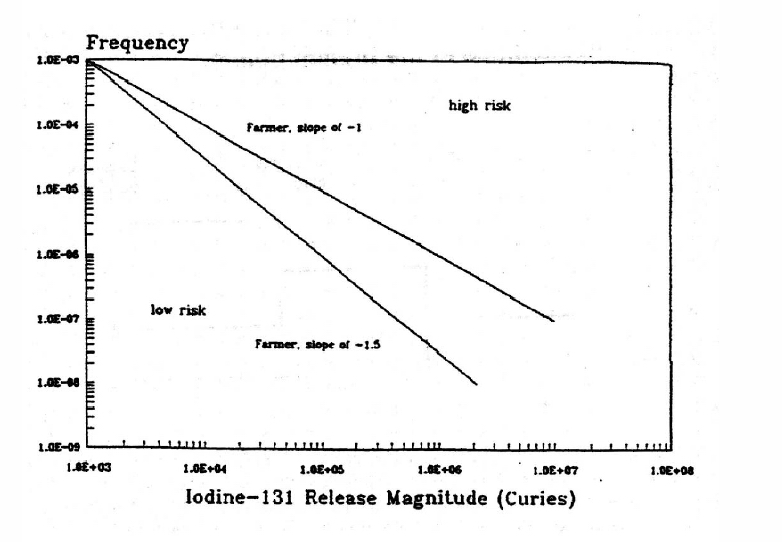
\includegraphics[width=0.75\textwidth]{farmers.chart.jpg}
%        \caption{}
    \end{figure}
\end{frame}


\begin{frame}{\href{https://radioactivity.eu.com/phenomenon/iodine_131}{I-131} is a major threat to health in a nuclear plant accident}
    \begin{enumerate}[series=outerlist,topsep=0pt,itemsep=15pt,leftmargin=*,label=(\arabic*)]
        \item[]Farmer considered the public acceptability of risk  
        \item[]Whole spectrum of events needs to be considered  
        \item[]Not just worst case (which would be low frequency)
        \item[]Low consequence but more probable carries equal risk
        \item[]Postulated a near-inverse for acceptable risk  
        \item[]Events with twice the consequence must be half as frequent
    \end{enumerate}
\end{frame}


\begin{frame}[plain]{}
    \centering\textbf{There are two overall `spaces' to consider with risk assessment}
\end{frame}


\addtocounter{framenumber}{-1}
\begin{frame}{1. After the accident}
    \begin{enumerate}[series=outerlist,topsep=0pt,itemsep=21pt,leftmargin=*,label=(\arabic*)]
        \item[]Figure out what went wrong
        \item[]Limit potential exposures and releases
        \item[]Prevent future similar accidents
        \item[]19.3 in the book
    \end{enumerate}
\end{frame}


\begin{frame}{2. Facility/process/experimental operations}
    \begin{enumerate}[series=outerlist,topsep=0pt,itemsep=11pt,leftmargin=*,label=(\arabic*)]
        \item[]Demonstrate ahead of time what the risks are and how they meet institutional requirements
        \item[]19.3.1. discusses again about the detection of small structural cracks in aircraft
        \item[]You can't really establish a probability of detection of the cracks
        \item[]But you can determine how experience would make detection more reliable
        \item[]Knowing what parts are more prone to cracks
        \item[]So you need qualitative efforts to determine this
        \item[]Develop a survey to determine experience level of inspectors
        \item[]Conduct a physical experiment to collect quantitative data from a lot of inspectors
    \end{enumerate}
\end{frame}


\begin{frame}[plain]{}
    \centering\LARGE\textbf{WASH-1400}
\end{frame}


\addtocounter{framenumber}{-1}
\begin{frame}{\href{https://uidaho.pressbooks.pub/riskassessment/chapter/pra-2/}{WASH-1400} came along in 1975}
    \begin{enumerate}[series=outerlist,topsep=0pt,itemsep=11pt,leftmargin=*,label=(\arabic*)]
        \item[]First formalized use of \acs{pra} -- Fault and events trees, etc.
        \item[]Dominant contributors to risk were small \acsp{loc} and transients
        \item[]Core damage frequency higher than what was thought at the time  
        \item[]But consquences smaller
        \item[]Support systems and operator actions very important
        \item[]Change in the reactor coolant system temperature, pressure, or both, attributed to a change in the reactor's power output
        \item[]300 reactor-years commercial experience
    \end{enumerate}
\end{frame}


\begin{frame}[plain]{}
    \centering\LARGE\textbf{WASH-1400 peer review}
\end{frame}


\addtocounter{framenumber}{-1}
\begin{frame}{WASH-1400 was \href{http://www.iaea.org/inis/collection/NCLCollectionStore/_Public/10/452/10452296.pdf}{reviewed by experts}}
    \begin{enumerate}[series=outerlist,topsep=0pt,itemsep=7pt,leftmargin=*,label=(\arabic*)]
        \item Clarify the achievements and limitations of WASH-1400
        \item Assess the peer comments thereon, and responses
        \item Study the present state of such risk assessment methodology
        \item Recommend to \acs{nrc} how (whether) such methodology can be used in the regulatory and licensing process
            \vspace{0.25in}
        \item[]
            \begin{quote}
                WASH-1400 was a conscientious and honest effort to apply the methods of fault-tree/event-tree analysis to an extremely complex system, a nuclear reactor, in order to determine the overall probability and consequences of an accident.
            \end{quote}
    \end{enumerate}
\end{frame}


\begin{frame}{They identified several problems we still talk about}
    \begin{enumerate}[series=outerlist,topsep=0pt,itemsep=17pt,leftmargin=*,label=(\arabic*)]
        \item[]
            \begin{quote}
                Inability to quantify human adaptability during the course of an accident
            \end{quote}
        \item[]
            \begin{quote}
                Inadequate treatment of common cause failure 
            \end{quote}
        \item[]
            \begin{quote}
                We are unable to define whether the overall probability of a core melt given in WASH-1400 is high or low, but we are certain that the error bands are understated. We cannot say by how much. Reasons for this include an inadequate data base, a poor statistical treatment, an inconsistent propagation of uncertainties throughout the calculation, etc.
            \end{quote}
        \item[]Even with all the operational history to drawn upon, they still have problems
    \end{enumerate}
\end{frame}


\begin{frame}{Risk assessment itself though was considered good}
    \begin{enumerate}[series=outerlist,topsep=0pt,itemsep=21pt,leftmargin=*,label=(\arabic*)]
        \item[]
            \begin{quote}
                We do find that the methodology, which was an important advance over earlier methodologies applied to reactor risks, is sound, and should be developed and used more widely under circumstances in which there is an adequate data base or sufficient technical expertise to insert credible subjective probabilities into the calculations.
            \end{quote}
        \item[]
            \begin{quote}
                The methodology can therefore provide a tool for the NRC to make the licensing and regulatory process more rational, in more properly matching its resources (research, quality assurance, inspection, licensing regulations) to the risks provided by the proper application of the methodology.
            \end{quote}
        \item[]
            \begin{quote}
                We find that the fault-tree/event-tree methodology is sound, and both can and should be more widely used by \acs{nrc}. The implementation of this methodology in WASH-1400 was a pioneering step, but leaves much to be desired.
            \end{quote}
    \end{enumerate}
\end{frame}


\begin{frame}{They didn't like how it was written}
    \begin{enumerate}[series=outerlist,topsep=0pt,itemsep=21pt,leftmargin=*,label=(\arabic*)]
        \item[]
            \begin{quote}
                It is very difficult to follow the detailed thread of any calculation through the report.
            \end{quote}
        \item[]
            \begin{quote}
                We find that the Executive Summary is a poor description of the contents of the report, should not be portrayed as such, and has lent itself to misuse in the discussion of reactor risks.
            \end{quote}
    \end{enumerate}
\end{frame}


\addtocounter{framenumber}{-1}
\begin{frame}{Other major findings}
    \small
    \begin{enumerate}[series=wash,topsep=0pt,itemsep=0pt,leftmargin=*,label=(\arabic*)]
        \item WASH-1400 was a substantial advance over previous attempts to estimate the risks of the nuclear option. The methodology has set a framework that can be used more broadly to assess choices involving both technical consequences and impacts on humans
        \item Made study of reactor safety more rational
        \item Established a topology of accident sequences
        \item Delineated procedures to quantify risk \textit{for those sequences for which a database exists}
        \item Error bounds may be understated due to inadequate database
        \item Inability to quantify common cause failures
        \item Inability to quantify human adaptability during the course of an accident (as illustrated at Browns Ferry) and failure to take credit for this is a major source of conservatism
        \item Transients, small \acs{loc}, and human errors are important contributors to overall risk, yet their study is not adequately reflected in the priorities of either the research or regulatory groups
        \item Most complete single picture of accident probabilities associated with nuclear reactors
        \item Fault/event tree approach coupled with an adequate data base is the best available tool with which to quantify these probabilities
        \item Made clear the importance to reactor safety discussions of accident consequences other than early fatalities (thyroid damage, land contamination, delayed cancers, genetic defects, etc.) for the first time
    \end{enumerate}
\end{frame}


\begin{frame}{Let's look at some recommendations}
    \begin{enumerate}[series=outerlist,topsep=0pt,itemsep=11pt,leftmargin=*,label=(\arabic*)]
        \item Incorporate lessons learned into \acs{nrc} licensing criteria
        \item Use \acs{pra} to reduce uncertainties
        \item Still use \acs{pra} even if data base is inadequate
        \item Use \acs{pra} for other electric generating technologies
        \item Fault/event tree analyses should be among the principal means used to deal with generic safety issues, to formulate new regulatory requirements, to assess and revalidate existing regulatory requirements, and to evaluate new designs
    \end{enumerate}
\end{frame}


\begin{frame}{And some limitations}
    \begin{enumerate}[series=outerlist,topsep=0pt,itemsep=11pt,leftmargin=*,label=(\arabic*)]
        \item Insufficient human data for the trees (though this seems at odds with what they just said)
        \item Methodological weakness due to the difficulty of incorporating time-window information into the event trees
        \item Humans might make things worse, which is hard to analyze
        \item But they might also make things better
        \item This leads to uncertainty in assessing human factors
            \vspace{0.10in}
        \item[]Recommend that the \acs{nrc} undertake a systematic program to evaluate the need for better human data
        \item[]Time dependencies only recently being addressed with dynamic risk assessment
    \end{enumerate}
\end{frame}


\begin{frame}{SHADE}
    \begin{quote}
        It must be said at the outset that RSS represents the fruits of a praiseworthy and pioneering effort to deal in depth with an extremely complex subject. It is a monumental report, written in three years by a large number of people and (although it is difficult to count the pages because they are not consecutively numbered) is nearly a foot thick. Clearly no one person can, or did, write all of this, and the report suffers thereby from incoherence.     
    \end{quote}
\end{frame}


\begin{frame}{A specific definition of risk was not defined }
    \begin{enumerate}[series=outerlist,topsep=0pt,itemsep=21pt,leftmargin=*,label=(\arabic*)]
        \item[]But displayed its results through graphs of the probability of occurrence of an event against the consequences of that event
        \item[]Other means of displaying the results could produce different risk perceptions
        \item[]We know that is the definition of risk now
    \end{enumerate}
\end{frame}


\begin{frame}{Establishing acceptable levels of risk is always challenging}
    \begin{enumerate}[series=outerlist,topsep=0pt,itemsep=21pt,leftmargin=*,label=(\arabic*)]
        \item[]WASH-1400 compared estimated risks with other societal risks in Chapters 6 and 7
        \item[]To judge acceptability of nuclear reactors solely on the risk of early fatalities, and latent health effects, and property damage for Class 9 accidents is inappropriate
        \item[]Public perception hangs heavily upon the perceived credibility of \acs{nrc}
        \item[]I'm actually surprised to see this statement and wonder how they arrived at it
    \end{enumerate}
\end{frame}


\begin{frame}{They also considered the effects of \href{https://youtu.be/z5rRZdiu1UE}{sabotage}}
    \begin{enumerate}[series=outerlist,topsep=0pt,itemsep=21pt,leftmargin=*,label=(\arabic*)]
        \item[]It is also worth noting that some features that make the plants difficult to sabotage successfully would also help to make most sabotage scenarios benign from the standpoint of public injury
        \item[]It would be-much easier to sabotage the plant so as to lead to shutdown and a need for expensive repair than to produce a core melt
        \item[]What about sabotage now? 
    \end{enumerate}
\end{frame}


\begin{frame}[plain]{}
    \centering\LARGE\textbf{Brown's Ferry}
\end{frame}


\addtocounter{framenumber}{-1}
\begin{frame}{Could \acs{pra} have predicted \href{http://www.ccnr.org/browns_ferry.html}{Brown's Ferry}?}
    \begin{enumerate}[series=outerlist,topsep=0pt,itemsep=21pt,leftmargin=*,label=(\arabic*)]
        \item[]March 1975  
        \item[]Two \acsp{bwr}
        \item[]Electricians were using \textit{candles} to test for air leaks and the sealant caught on fire
        \item[]Common cause failures in a variety of otherwise independent and redundant systems
        \item[]Control of 11 relief valves lost  
        \item[]Only source of makeup water was a control rod drive pump not intended for this purpose and of inadequate capacity for the long term
    \end{enumerate}
\end{frame}


\begin{frame}{Nothing actually went wrong}
    \begin{enumerate}[series=outerlist,topsep=0pt,itemsep=15pt,leftmargin=*,label=(\arabic*)]
        \item[]Valves were repaired in 5 and a half hours 
        \item[]Reactor shutdown safely
        \item[]\href{https://www.osti.gov/biblio/7327154}{Appendix XI} of WASH-1400 contains a probabilistic analysis of the Browns Ferry event
        \item[]Failed to estimate that last 4 valves would fail because air supply ran out  
        \item[]No models for repair times
        \item[]Reviewers don't comment on whether the core melt probability is reasonable
        \item[]Aren't particularly glowing of the assessment either  
        \item[]Do not think \acs{pra} captured fire as an important accident initiator
    \end{enumerate}
\end{frame}


\begin{frame}{The accident was initiated by human error}
    \begin{enumerate}[series=outerlist,topsep=0pt,itemsep=15pt,leftmargin=*,label=(\arabic*)]
        \item[]Which is still hard to model
        \item[]
            \begin{quote}
                A a substantial element of conservatism in the body of WASH-1400 (other than in the analysis of Browns Ferry) lies in failing to take credit for the fact that well-trained humans provide adaptive coping capability.
            \end{quote}
        \item[]This is similarly hard to model or quantify
        \item[]
            \begin{quote}
                Too little time and energy have been expenaed in using the event to help quantify some of the inputs to a reactor safety analysis which are most difficult to quantify: quality assurance, human behavior, common cause failure, etc. It is even now not too late for the NRC to have some impartial body do these things.
            \end{quote}
        \item[]So, the same things as now 
    \end{enumerate}
\end{frame}


\begin{frame}[plain]{}
    \centering\LARGE\textbf{Common cause failures}
\end{frame}


\addtocounter{framenumber}{-1}
\begin{frame}{Can \acs{pra} identify common cause failures?}
    \begin{enumerate}[series=outerlist,topsep=0pt,itemsep=21pt,leftmargin=*,label=(\arabic*)]
        \item[]Common cause failure may invalidate some of the sequential features of an event-tree, while at the same time causing failures on adjacent and apparently disparate event-trees (report)
        \item[]With so many people working on all the event trees, it's easy to see how common cause failures could slip through (me) 
        \item[]
            \begin{quote}
                We are unconvinced by the arguments for completeness of the report in connection with common cause failures.
            \end{quote}
        \item[]Common cause failures can activate low probability accident sequences that would otherwise be overlooked
        \item[]So this continues to be a problem with \acs{pra}
    \end{enumerate}
\end{frame}


\begin{frame}{Principal assurance against common cause failures must lie in dealing with initiating events}
    \begin{enumerate}[series=outerlist,topsep=0pt,itemsep=11pt,leftmargin=*,label=(\arabic*)]
        \item Fire
        \item Earthquakes
        \item Acts of violence
        \item Explosions and missiles
        \item Massive electrical failure
        \item Human error
        \item Flood, tsunamis
        \item Tornadoes, hurricanes
            \vspace{0.10in}
        \item[]How do you mitigate these initating events?
    \end{enumerate}
\end{frame}


\begin{frame}{Earthquake is potential initiator of a common cause failure}
    \begin{enumerate}[series=outerlist,topsep=0pt,itemsep=21pt,leftmargin=*,label=(\arabic*)]
        \item[]WASH-1400 found earthquakes to be small contributors to the total risks of core melt
        \item[]Earthquake risk in nuclear plants deserves much more attention than it has received
        \item[]Investigation at a level of sophistication necessary to resolve issue to our satisfaction has not yet been performed, and it is important that done
    \end{enumerate}
\end{frame}


\begin{frame}{}
    \begin{figure}
        \centering
        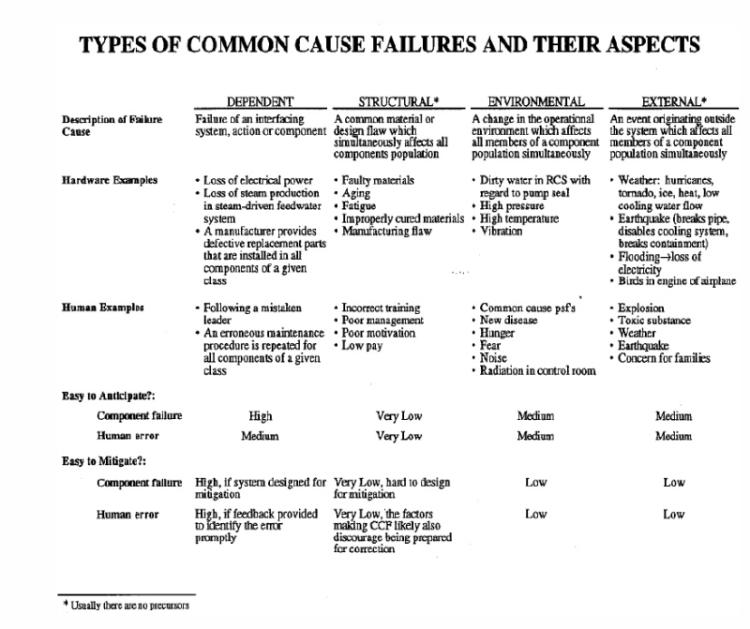
\includegraphics[width=0.70\textwidth]{common.cause.failures.jpg}
%        \caption{}
    \end{figure}
\end{frame}


\begin{frame}[plain]{}
    \centering\LARGE\textbf{Human factors}
\end{frame}


\addtocounter{framenumber}{-1}
\begin{frame}{People screwing up also cause a lot of accidents}
    \begin{enumerate}[series=outerlist,topsep=0pt,itemsep=7pt,leftmargin=*,label=(\arabic*)]
        \item[]Which is why we have the human factors field
        \item[]The peer review group was not pleased about the lack of peer comment on human factors
        \item[]But no one had any expertise in it either 
            \vspace{0.10in}
        \item Humans operate systems during an accident to mitigate consequences
        \item Humans can make a mistakee to aggravate the situation
        \item Accidents can be initiated by humans through error
        \item Humans can inadvertantly disable safety equipment that will then be unavilable in an accident
    \end{enumerate}
\end{frame}


\begin{frame}{Event and fault trees must take human intervention into account}
    \begin{enumerate}[series=outerlist,topsep=0pt,itemsep=21pt,leftmargin=*,label=(\arabic*)]
        \item Human performance data base is weak (at the time)
        \item Human factor data used in WASH came from nonnuclear experience
        \item Event/fault trees need to be highly detailed
        \item Some human-intertention phenomena are time-dependent (hard to quantify)
        \item Uncertainties arise when expert judgment is used 
    \end{enumerate}
\end{frame}


\begin{frame}{WASH1400 threw human factors a bone}
    \begin{enumerate}[series=outerlist,topsep=0pt,itemsep=21pt,leftmargin=*,label=(\arabic*)]
        \item Role of operators delinated better than prior to WASH1400
        \item Experience with other highly complex systems operated by well trained personnels is relevant
        \item Consensus among other experts WASH1400 estimated human error well
        \item[]But they point out that a substantive review did not occur
    \end{enumerate}
\end{frame}


\begin{frame}[plain]{}
    \centering\LARGE\textbf{Quantitative comparisons}
\end{frame}


\addtocounter{framenumber}{-1}
\begin{frame}{}
    \begin{figure}
        \centering
        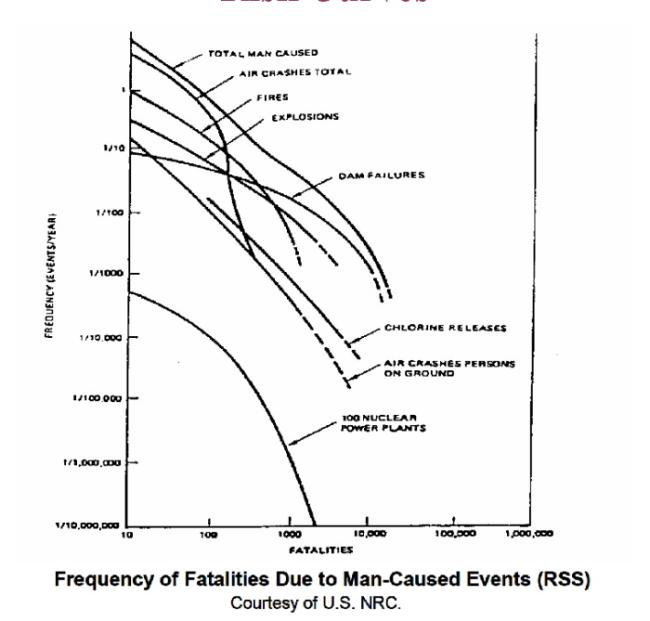
\includegraphics[width=0.60\textwidth]{wash.farmer.jpg}
%        \caption{}
    \end{figure}
\end{frame}


\begin{frame}[plain]{}
    \centering\LARGE\textbf{Follow up to WASH-1400}
\end{frame}


\addtocounter{framenumber}{-1}
\begin{frame}{Zion and Indian Point were the first \acsp{pra} sponsored by industry}
    \begin{enumerate}[series=outerlist,topsep=0pt,itemsep=21pt,leftmargin=*,label=(\arabic*)]
        \item[]Comprehensive analysis of uncertainties (Bayesian methods)
        \item[]Detailed containment analysis (not all accidents lead to containment failure)
        \item[]`External' events (earthquakes, fires) may be significant contributors to risk
        \item[]Still have not found these \href{https://www.ans.org/news/article-3693/perspectives-from-past-nrc-commissioners/}{reports}
    \end{enumerate}
\end{frame}


\begin{frame}{The follow up to WASH1400 was \href{https://uidaho.pressbooks.pub/riskassessment/chapter/pra-2/}{NUREG1150} 1990}
    \begin{enumerate}[series=outerlist,topsep=0pt,itemsep=21pt,leftmargin=*,label=(\arabic*)]
        \item[]Average probability of an individual early fatality per reactor per year
        \item[]\acs{nrc} Safety Goal -- $5 \times 10^{-7}$
        \item[]Level I \acs{pra} methods generally sound
        \item[]Concerns with human reliability analysis, common cause failures, data analysis
        \item[]Same things we talk about today
    \end{enumerate}
\end{frame}


\begin{frame}{}
    \begin{figure}
        \centering
        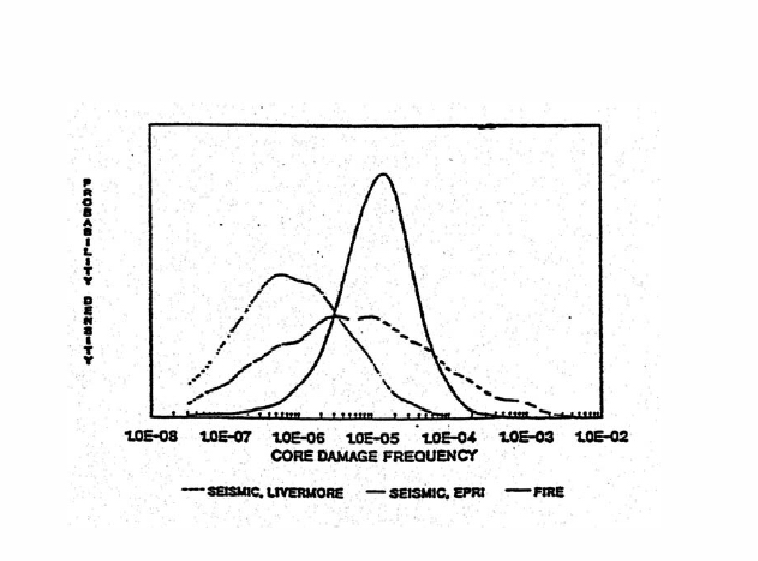
\includegraphics[width=0.80\textwidth]{cdf.jpg}
%        \caption{}
    \end{figure}
\end{frame}


\begin{frame}{}
    \begin{figure}
        \centering
        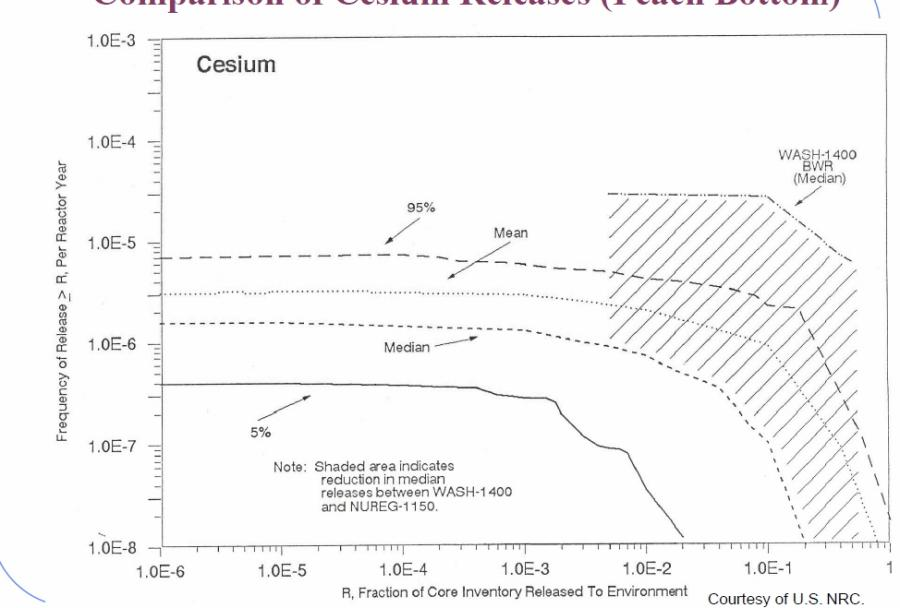
\includegraphics[width=0.80\textwidth]{cesium.release.jpg}
%        \caption{}
    \end{figure}
\end{frame}


\begin{frame}{}
    \begin{figure}
        \centering
        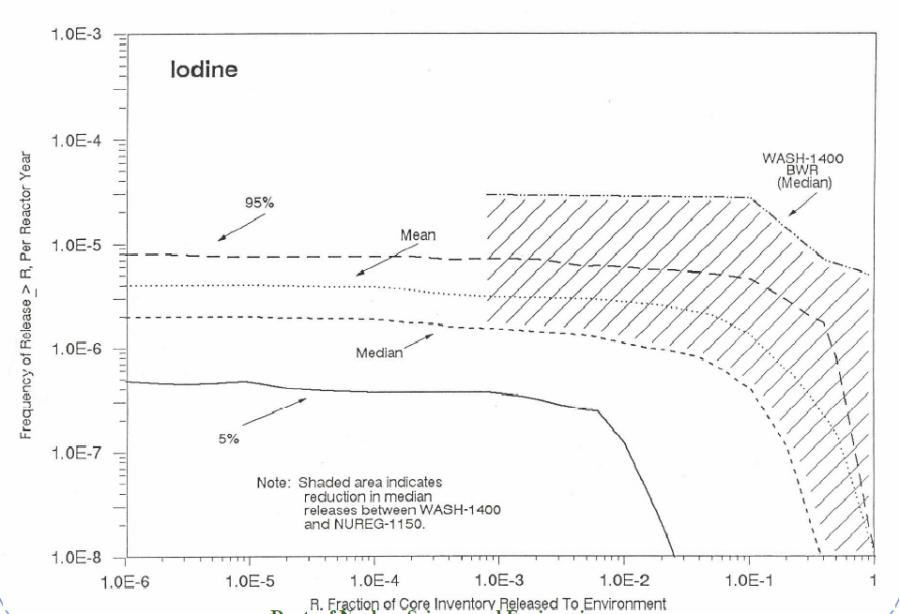
\includegraphics[width=0.80\textwidth]{iodine.release.jpg}
%        \caption{}
    \end{figure}
\end{frame}


\begin{frame}[plain]{}
    \centering\LARGE\textbf{1995 Policy statement}
\end{frame}


\addtocounter{framenumber}{-1}
\begin{frame}{\acs{nrc} released a \href{https://www.nrc.gov/about-nrc/regulatory/risk-informed/history.html}{policy statement} 1995}
    \begin{enumerate}[series=outerlist,topsep=0pt,itemsep=17pt,leftmargin=*,label=(\arabic*)]
        \item[]Use of \acs{pra} should be increased to the extent supported by the state of the art and data and in a manner that complements the defense-in-depth philosophy
        \item[]\acs{pra} should be used to reduce unnecessary conservatisms associated with current regulatory requirements
        \item[]This is still kind of a problem
        \item[]Insights derived from \acsp{pra} are used in combination with deterministic system analysis to focus licensee and regulatory attention on issues commensurate with their importance to safety
        \item[]Use risk to inform decision making, not dictate the decision
        \item[]Measurable parameters monitor plant and licensee performance
    \end{enumerate}
\end{frame}


\begin{frame}{Devise objective criteria to assess system performance }
    \begin{enumerate}[series=outerlist,topsep=0pt,itemsep=17pt,leftmargin=*,label=(\arabic*)]
        \item[]Based on a combination of risk insights, deterministic analysis, and performance history  
        \item[]Licensee flexibility to determine how to meet established performance criteria
        \item[]Failure to meet a performance criterion must not result in unacceptable consequences
        \item[]\acs{npp} needs to make sure when an earthquake hits that there is no care damage or release  
        \item[]But how a CA plant does that v an MA plant is different
        \item[]Risk informed, performance based regulations 
    \end{enumerate}
\end{frame}


\begin{frame}[plain]{}
    \centering\LARGE\textbf{\acs{pra} challenges}
\end{frame}


\addtocounter{framenumber}{-1}
\begin{frame}{Doing a \acs{pra} is wicked hard}
    \begin{enumerate}[series=outerlist,topsep=0pt,itemsep=17pt,leftmargin=*,label=(\arabic*)]
        \item[]Models the whole system including hardware failures, human performance, and relevant physical phenomena
        \item[]Which is why you need all these tools
        \item[]When do you know the \acs{pra} is satisfactory, complete, comprehensive?
        \item[]Knowing a priori is highly subjective and very difficult
        \item[]Unknown unknowns
        \item[]Still a reactive process
    \end{enumerate}
\end{frame}


\begin{frame}{Failures result from events exhibiting dependencies}
    \begin{enumerate}[series=outerlist,topsep=0pt,itemsep=21pt,leftmargin=*,label=(\arabic*)]
        \item[]Or from a single shared cause and coupling factor
        \item[]Sequence of item failures where the first failure shifts its load to one or more nearby items
such that these fail and again shift their load to other item, etc.
        \item[]Cascade
        \item[]Why did the item fail?  
        \item[]Why were several items affected?
    \end{enumerate}
\end{frame}


\begin{frame}{Identify causes as part of facility or system design}
    \begin{enumerate}[series=outerlist,topsep=0pt,itemsep=21pt,leftmargin=*,label=(\arabic*)]
        \item[]Pre-operational causes stem from design, manufacturing, construction, installation
        \item[]Operational causes stem from inadequate maintenance and operational procedures, execution, competence, scheduling
        \item[]Redundancy and diversity  
        \item[]Isolation (shielding, containment, separation)
        \item[]There's lots of modeling for this (bayes and binomial distribution, tables)
    \end{enumerate}
\end{frame}


\begin{frame}[plain]{}
    \centering\LARGE\textbf{Putting it all together}
\end{frame}


\addtocounter{framenumber}{-1}
\begin{frame}{\acs{pra} was used by aviation and nuclear industry first, but now everyone uses it}
    \begin{enumerate}[series=outerlist,topsep=0pt,itemsep=15pt,leftmargin=*,label=(\arabic*)]
        \item[]Requires in-depth knowledge of the system or process  
        \item[]Tools like fault/event trees, \acs{pha}, \acs{haz}, \acs{fma} all contribute
        \item[]We need to know what normal operation looks like
        \item[]Identify deviations
        \item[]Assign frequencies (with uncertainties)
        \item[]Sensitivity analysis (\acs{haz})
    \end{enumerate}
\end{frame}


\begin{frame}{Integrate all our tools to assess risk}
    \begin{enumerate}[series=outerlist,topsep=0pt,itemsep=21pt,leftmargin=*,label=(\arabic*)]
        \item[]Identify end states  
        \item[]How can radiation be released?  
        \item[]How could people become exposed?  
        \item[]How could we lose a lot of money?
        \item[]Characterize the system comprehensively   
        \item[]You've all done some of this with all the homework projects
    \end{enumerate}
\end{frame}


\begin{frame}{Identify what data is going to be needed and how you would collect it}
    \begin{enumerate}[series=outerlist,topsep=0pt,itemsep=11pt,leftmargin=*,label=(\arabic*)]
        \item[]Select initiating events (hazards)
        \item[]Define scenarios linking each initiating event to the end states  
        \item[]Apply the trees, \acs{fma}, \acs{haz}
        \item[]Modeling where needed  
        \item[]Material flow models  
        \item[]Transport models  
        \item[]Quantify risk for each initiating event  
        \item[]Uncertainty and sensitivity analysis
    \end{enumerate}
\end{frame}


\begin{frame}{Rank risk}
    \begin{enumerate}[series=outerlist,topsep=0pt,itemsep=21pt,leftmargin=*,label=(\arabic*)]
        \item[]Farmers chart
        \item[]Regulations
        \item[]Peer review
        \item[]Management
    \end{enumerate}
\end{frame}


\begin{frame}{We have been focused largely on qualitative risk analysis}
    \begin{enumerate}[series=outerlist,topsep=0pt,itemsep=17pt,leftmargin=*,label=(\arabic*)]
        \item[]Risk assessment matrices 
        \item[]Being able to do this is most of the job
        \item[]Eventually, frequencies have to be developed
        \item[]Parameters quantified with associated uncertainties
        \item[]Models defined
        \item[]More specific to the system to be analyzed
    \end{enumerate}
\end{frame}


\begin{frame}[plain]{}
    \centering\LARGE\textbf{Narrative research}
\end{frame}


\addtocounter{framenumber}{-1}
\begin{frame}{Narrative research can be used to determine what happened}
    \begin{enumerate}[series=outerlist,topsep=0pt,itemsep=17pt,leftmargin=*,label=(\arabic*)]
        \item[]Way of understanding experience
        \item[]Determining risk by looking at an event such as an airplane crash
        \item[]You already did this for several examples
        \item[]Narrative research incorporates personal observation, records, videos, pictures
        \item[]Mitigate risk for future events
        \item[]Again, still a retrospective process though
    \end{enumerate}
\end{frame}


\begin{frame}{Quantitative risk analysis is needed for the Farmer's chart and regulations}
    \begin{enumerate}[series=outerlist,topsep=0pt,itemsep=15pt,leftmargin=*,label=(\arabic*)]
        \item[]Ultimately needed for Level I,II,III \acs{pra}
        \item[]We have initiating events and scenarios, including human effects
        \item[]We know how to obtain failure rates and process data
        \item[]Higher level statistical analysis used
        \item[]Like Monte Carlo
        \item[]Identify distributions for relevant parameters
        \item[]Run the model
        \item[]Establish confidence limits
    \end{enumerate}
\end{frame}


\begin{frame}[plain]{}
    \centering\LARGE\textbf{Case studies}
\end{frame}


\addtocounter{framenumber}{-1}
\begin{frame}{Case study research can be used to apply a bounded system to other problems}
    \begin{enumerate}[series=outerlist,topsep=0pt,itemsep=15pt,leftmargin=*,label=(\arabic*)]
        \item[]Hyatt
        \item[]Pinto $\rightarrow$ GM ignition
        \item[]Dreamliner
        \item[]Bay bridge
        \item[]Nuclear accidents
        \item[]Takata air bags
        \item[]Doesn't need to be historical
    \end{enumerate}
\end{frame}


\begin{frame}{Pedagogically, you want to teach fundamental principles, existing case studies}
    \begin{enumerate}[series=outerlist,topsep=0pt,itemsep=21pt,leftmargin=*,label=(\arabic*)]
        \item[]Then develop your own
        \item[]So data gathering (what/importance) is important because you aren't modeling on your own, or using existing data in a model to further analyze the case
    \end{enumerate}
\end{frame}


\begin{frame}{Consider repository assessment}
    \begin{enumerate}[series=outerlist,topsep=0pt,itemsep=21pt,leftmargin=*,label=(\arabic*)]
        \item[]Wide variety of engineering and scientific disciplines to be needed
        \item[]Geology, chemical engineering, environmental science, nuclear engineering
        \item[]Even though we've been working on small-scale projects, you should be able to expand to this level
        \item[]What is important is that risk has to be defined clearly for each system
    \end{enumerate}
\end{frame}


\begin{frame}[plain]{}
    \begin{figure}
        \centering
        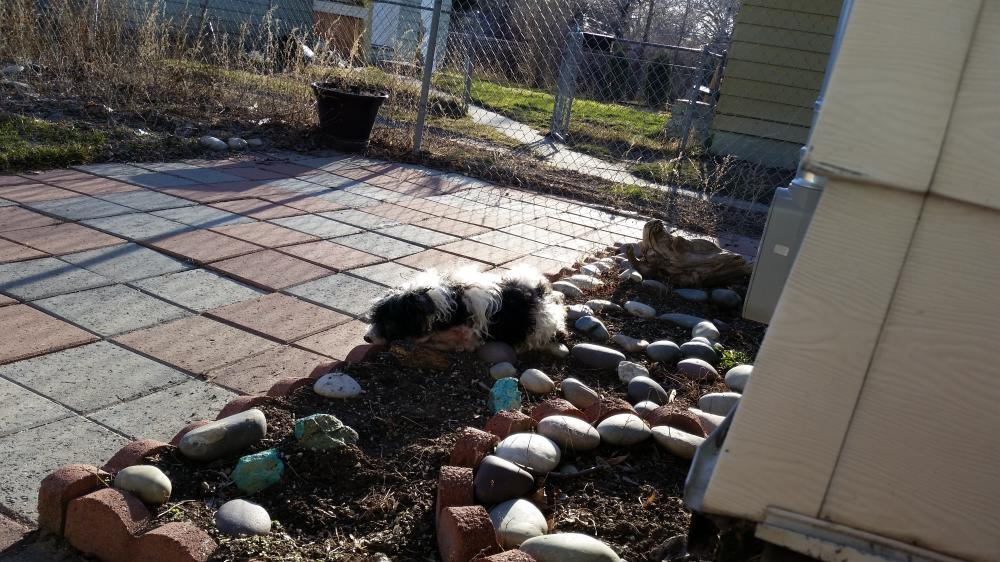
\includegraphics[width=0.85\textwidth]{final.jpg}
%        \caption{}
    \end{figure}
\end{frame}


%%%%%%%
%\begin{frame}{}
%    \begin{columns}
%
%        \begin{column}{0.50\textwidth}
%            \begin{enumerate}[series=outerlist,topsep=0pt,itemsep=21pt,leftmargin=*,label=(\arabic*)]
%                \item[]
%                \item[]
%            \end{enumerate}
%        \end{column}
%
%        \begin{column}{0.50\textwidth}
%            \begin{enumerate}[series=outerlist,topsep=0pt,itemsep=21pt,leftmargin=*,label=(\arabic*)]
%                \item[]
%                \item[]
%            \end{enumerate}
%        \end{column}
%
%    \end{columns}
%\end{frame}

%    \begin{figure}
%        \centering
%        \includegraphics[width=0.75\textwidth]{wsc.png}
%        \caption{\acs{wsc}}
%    \end{figure}


%\begin{frame}{References}
%    \bibliographystyle{nsf}
%    \footnotesize
%    \bibliography{references}
%\end{frame}
%%%%%%%


\end{document}
